\documentclass{article}
\usepackage[utf8]{inputenc}
\newcommand\tab[1][1cm]{\hspace*{#1}}
\DeclareRobustCommand\iff{\;\Longleftrightarrow\;}

\title{Tutoriat 8 - Rezolvări \\
\Large  Inele. Polinoame. }
\date{- 13 ianuarie 2021 -}
\author{Savu Ioan Daniel, Tender Laura-Maria}

\usepackage{natbib}
\usepackage{graphicx}
\usepackage{url}
\usepackage{amsmath}
\usepackage{amssymb}
\setcounter{secnumdepth}{0}
\begin{document}

\maketitle
\section{Exercițiul 1}
Arătați că:
\begin{itemize}
    \item $\mathbf{Q}[X]/(X^2-1) \cong \mathbf{Q} \times \mathbf{Q}.$
    \item $\mathbf{Z}[X]/(X^2-X) \cong \mathbf{Z} \times \mathbf{Z}.$
    \item $\mathbf{Z}[X]/(X^2-1) \ncong \mathbf{Z} \times \mathbf{Z}.$
\end{itemize}
\subsection{Rezolvare}
\begin{itemize}
    \item Putem rescrie $\mathbf{Q}[X]/(X^2-1) \cong \mathbf{Q}[X]/((X-1)(X+1)).$ Pentru a arăta că $(X - 1)$ și $(X + 1)$ sunt comaximale, trebuie să arătăm că suma lor genereazä tot $\mathbf{Q}[X]$. Este suficient să arătåm că suma idealelor conține elementul unitate. \newline \newline
Observăm că $(X + 1) - (X - 1) = 2$. Înmulțind relația cu $\frac{1}{2}$ (putem face această operație întrucât lucrăm în mulțimea numerelor raționale) obținem 1. \newline \newline
$\mathbf{Q}[X]/((X-1)(X+1)) \cong \mathbf{Q}[X]/(X-1)\cap (X+1)$ \newline
$\mathbf{Q}[X]/(X-1)\cap (X+1) \cong \mathbf{Q}[X]/(X-1)\times \mathbf{Q}[X]/(X+1)$ \newline \newline
Clasele de echivalență ale lui $\mathbf{Q}[X]/(X-1)$ sunt resturile obținute prin împărțirea oricărui polinom la $X-1$, deci sunt polinoame de grad 0, de forma $\{a \ | a \in \mathbf{Q} \}$, deci $\mathbf{Q}[X]/(X-1)\cong \mathbf{Q}$. Analog pentru $\mathbf{Q}[X]/(X+1)\cong \mathbf{Q}$ \newline \newline
În concluzie, $\mathbf{Q}[X]/(X^2-1) \cong \mathbf{Q} \times \mathbf{Q}.$
\item Demonstrația decurge asemănător pentru $\mathbf{Z}[X]/(X^2-X)$, cu observația că $X^2-X = X(X-1)$. Sunt comaximale deoarece $X - (X-1) = 1$.
\item Spre deosebire de primul subpunct, aici nu mai putem înmulți relația cu $\frac{1}{2}$, întrucât lucrăm cu mulțimea numerelor întregi. \newline
Presupunem că inelul factor ar fi izomorf cu $\mathbf{Z} \times \mathbf{Z}$. Ne uităm la elementele idempotente ale acestor două inele.\newline
Observație: deoarece $X^2-1$ aparține idealului prin care factorizăm,
 $\widehat{X^2-1} = \widehat{0}$, de unde $\widehat{X^2} = \widehat{1}$. \newline
 Fie $\widehat{a}X + \widehat{b}$ un element indempotent. \newline
 Atunci $(\widehat{a}X + \widehat{b})^2 = \widehat{a}X + \widehat{b}$,  $\widehat{a}^2 X^2 + 2\widehat{ab}X + \widehat{b}^2 = \widehat{a}X + \widehat{b}$, $\widehat{a}^2 + 2\widehat{ab}X + \widehat{b}^2 = \widehat{a}X + \widehat{b}$. \newline \newline
 $\begin{cases} 
 \widehat{a}^2 +  \widehat{b}^2 = \widehat{b}\\ 
 2\widehat{ab} = \widehat{a}
 \end{cases}$
 Singurele soluții ale ecuațiilor în $\mathbf{Z}$ sunt $a = 0$ și $b \in \{0,1\}$. Deci obținem 2 elemente indempotente. \newline
 În $\mathbf{Z} \times \mathbf{Z}$, sunt 4 elemente idempotente: $\{(0,0), (0,1), (1, 0), (1, 1)\}$. Având număr diferit de idempotenți, inelele nu sunt izomorfe.
 
\end{itemize}

\section{Exercițiul 2}
Fie idealul $I = (X^3, X^5)$ al inelului de polinoame $\mathbf{Q}[X]$.
\begin{enumerate}
    \item Dați un exemplu de polinom care aparține lui $I$ și are 4 termeni nenuli.
    \item Dați un exemplu de polinom care nu aparține lui $I$ și are 3 termeni nenuli.
    \item Este adevărat că $I=(X^3)$? Dar că $I=(X^5)$? Justificați.
    \item Determinați elementele nilpotente din inelul factor $\mathbf{Q}[X]/I$.
    \item Determinați elementele idempotente din inelul factor $\mathbf{Q}[X]/I$.
    \item Sunt izomorfe inelele $\mathbf{Q}[X]/I$ și $\mathbf{Q} \times \mathbf{Q}$?. Justificați.
\end{enumerate}  
\subsection{Rezolvare}
(1) Cum $X^5 \in I$, un astfel de polinom este $X^5 + X^6 + X ^ 7 + X^8$.
\newline
(2) Fie $P=X^2 + X^1 + 1$. Presupunem ca $P \in I$. Atunci $P = X^3 * A + X^5 * B$, unde $A, B$ sunt polinoame. Observăm că $P$ poate fi rescris ca $P=X^3*C$, cu $C$ polinom. Comparând gradele posibile pentru $X^3*C$ și pentru P, rezultă că $P$ nu poate fi egal cu $X^3*C$. Contradicție. Prin urmare $P \not \in I$ și $P$ are 3 termeni nenuli, deci este un polinom valid pentru cerință.
\newline
(3) Orice polinom din $I$ poate fi scris sub forma $X^3 * A + X^5 * B$ cu $A, B$ polinoame. Astfel, aranjând termenii, putem scrie mai departe că un polinom din $I$ este de forma $X^3*C$ cu $C$ polinom. Putem observa imediat că $I=(X^3)$. De asemenea, din ultima relație, avem că $I \not = (X^5)$ deoarece $I=(X^3)$ și $X^3 \in (X^3)$ dar $X^3 \not \in (X^5)$.
\newline
(4) Elementele din grupul factor sunt de forma $P=\widehat{aX^2 + bX + c} = \widehat{X(b+aX) + c},$ cu $a, b, c \in \mathbf{R}.$ P este nilpotent daca $\exists n \in \mathbf{N}$ a.î. $P^n$ este multiplu de $X^3$. Din ultima relație, daca scriem $P^n$ folosind binomul lui Newton observăm ca acesta este multiplu de $X^3 \iff c = 0$. Prin urmare, există o infinitate de elemente nilpotente, acestea fiind de forma $aX^2 + bX$.
\newline
(5) Analog subpunctului anterior, $P=\widehat{ax^2 + bX + c}$. Trebuie să rezolvăm ecuația $P^2 = P$, de unde $(b^2 + 2ac)X^2 + 2bcX + c^2 = aX^2 + bX + c$. Avem două soluții, și anume $0$ și $1$ care sunt idempotenții triviali. Prin urmare, idempotenții inelului factor sunt idempotenții triviali.
\newline
(6) În $\mathbf{Q} \times \mathbf{Q}$ singurul element nilpotent este $(0, 0)$. În inelul factor, conform (4), există o infinitate de elemente nilpotente. Prin urmare, cele două inele nu pot fi izomorfe.


\section{Exercițiul 3}
Fie polinomul $P(X) = X^4 - X^2 + 1$ având rădăcinile complexe $\alpha_1, ..., \alpha_4$.
\begin{enumerate}
    \item  Descompuneți polinomul $P(X)$ în factori ireductibili peste fiecare dintre corpurile $\mathbf{R}, \, \mathbf{Q}, \, \mathbf{Z}_2, \, \mathbf{Z}_3$.
    \item Calculați $\alpha_1^5 + ... + \alpha_4^5$.
    \item Determinați explicit coeficienții unui polinom nenul care să aibă ca rădăcini pe $2 \alpha_1 - 1 , ..., 2 \alpha_4 - 1$.
\end{enumerate}

\subsection{Rezolvare}
\begin{enumerate}
    \item $P(X) = X^4 - X^2 + 1 = X^4 + 1 - X^2 = X^4 + 2X^2 + 1 - 3X^2 = (X^2 + 1)^2 - 3X^2 = (X^2 + 1 - \sqrt{3}X)(X^2 + 1 + \sqrt{3}X)$.\newline
    Știm că un polinom este ireductibil peste $\mathbf{C}$, dacă este descompus în polinoame de gradul întâi. Însă, peste $\mathbf{R}$, un polinom este ireductibil dacă este descompus în polinoame de gradul întâi sau în polinoame de gradul al doilea cu $\Delta < 0$. \newline
    Calculăm $\Delta$ pentru cele două polinoame de gradul al doilea în care lam descompus pe $P(X)$. $\Delta_1 = \Delta_2 =  3 - 4 = -1 < 0$. Deci forma este ireductibilă peste $\mathbf{R}$. \newline
    Vom arăta că $P(X)$ este ireductibil peste $\mathbf{Q}$. Presupunem că există $\frac{m}{n}, (m, n) = 1, m \in \mathbf{Z}, n \in \mathbf{N}^*$ astfel încât $P(\frac{m}{n}) = 0$, $\frac{m}{n}$ rădăcină a lui $P(X)$. \newline
    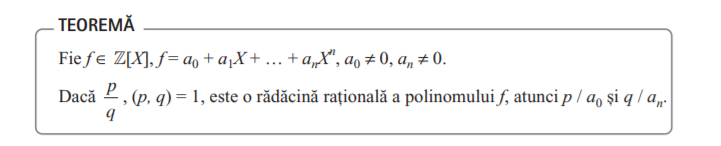
\includegraphics[width = \textwidth]{teorema.PNG}
    \newline
    Atunci $m|1$ și $n|1$, deci $\frac{m}{n} \in \{+1, -1\}$. \newline
    $P(1) = 1 \neq 0, P(-1) = 1 \neq 0$. Astfel, presupunerea făcută este falsă, deci $P(X)$ este ireductibil peste $\mathbf{Q}$. \newline
    Peste $\mathbf{Z}_2$, $P(X) = X^4 + X^2 + 1 = (X^2 + X + 1)^2. f(X) = (X^2 + X + 1)^2. f$ este ireductibil peste $\mathbf{Z}_2$ întrucât $f(\widehat{0}) = \widehat{1}$ și $f(\widehat{1}) = \widehat{1}$. \newline
    Peste $\mathbf{Z}_3$, $P(X) = X^4 + \widehat{2}X + \widehat{1} = (X^2 + \widehat{1})^2. \ X^2 + \widehat{1}$ este ireductibil peste $\mathbf{Z}_3$.  
    \item $P(\alpha_i) = 0, \, i \in \overline{(1, 4)}.$ Deci $\alpha_i^4 - \alpha_i^2 + 1 = 0 \iff \alpha_i^4 = \alpha_i^2 - 1$. \newline
    $\alpha_i^5 = \alpha_i^3 - \alpha_i$. $\sum_{i=1}^{4} \alpha_i^5 = \sum_{i=1}^{4} \alpha_i^3  - \sum_{i=1}^{4} \alpha_i$ \newline
    Conform relațiilor lui Viete, $s_1 = p_1 = \sum_{i=1}^{4} \alpha_i = 0$. $s_2 = -1, s_3 = 0, s_4 = 1.$ Dorim să aflăm $p_3 = \sum_{i=1}^{4} \alpha_i^3$. Conform formulelor lui Newton \newline
    $p_3 - p_2 s_1 + p_1 s_2 - 3s_3 = 0$ \newline
    $p_1 = s_1 = 0 \Rightarrow p_3 = 3s_3 = 0$ \newline
    În concluzie, $\sum_{i=1}^{4} \alpha_i^5 = 0$.
    \item
    $2\alpha_i - 1 = \beta_i \iff  \alpha_i = \frac{\beta_i + 1}{2}$ \newline
    Răspunsul este polinomul $Q(X) = P(\frac{X + 1}{2}) = (\frac{X + 1}{2})^4 -  (\frac{X + 1}{2})^2 + 1.$
\end{enumerate}   

\end{document}
